\section{Automatic partitioning}\textit{"Automatic partitioning"} deletes all data from the client hard disk. m23 will create two new partitions, one for the data and base system and one for swapping.\\
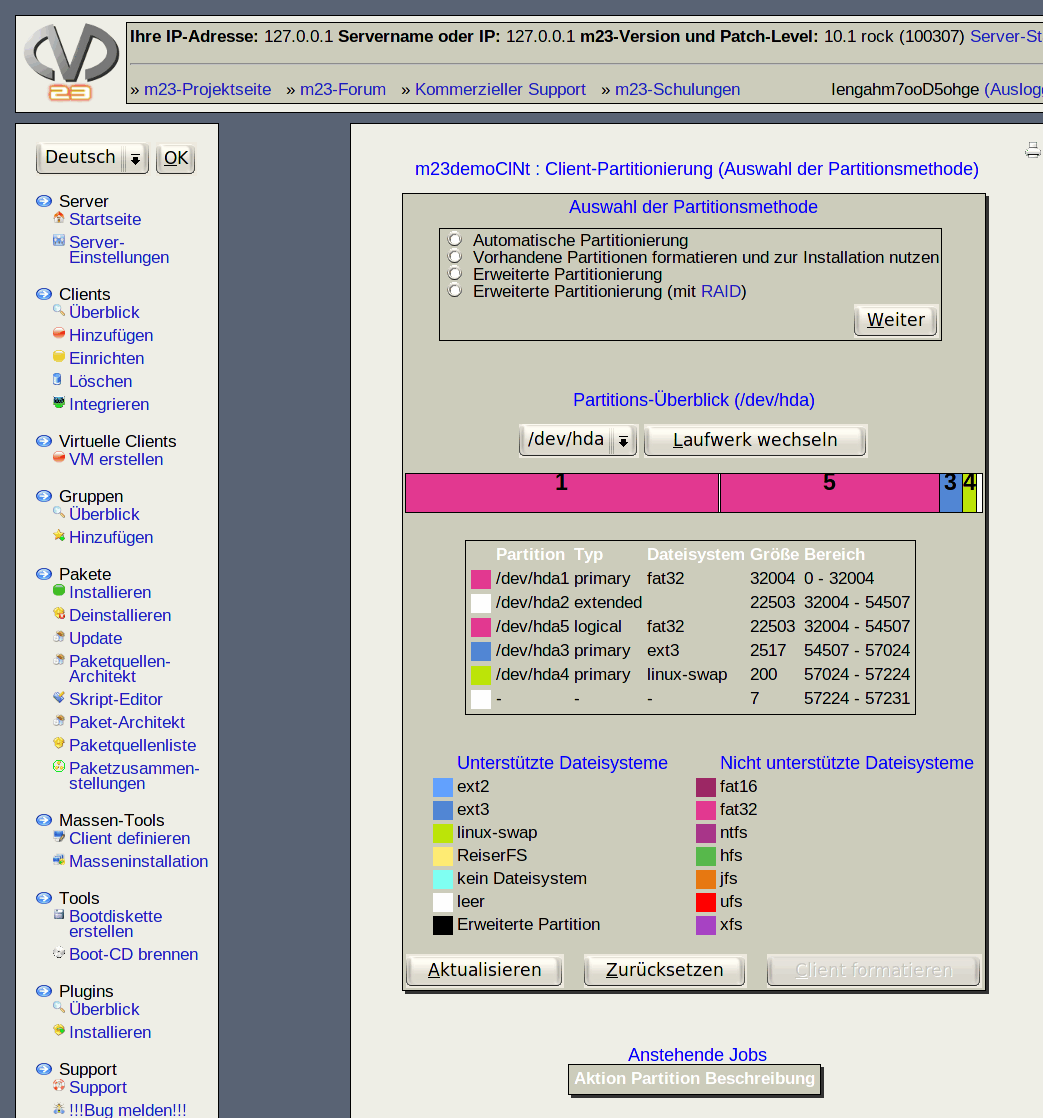
\includegraphics[scale=0.4]{/mdk/doc/manual/screenshots/en/fdisk-automatic.png} \\
\subsection{Step by step:}
\begin{enumerate}
\item Select \textit{"Automatic partitioning"}.\\
\item Click on the \textit{"Refresh"} button to see the suggested partitioning.\\
\item Click on \textit{"Format client"} to accept changes.\\
\end{enumerate}
